\documentclass[aspectratio=169,10pt]{beamer}

% ---------------------------------------------------------------------------
% A self-contained tutorial on connecting tools and knowledge to an LLM.
% ---------------------------------------------------------------------------

\usetheme{Madrid}
\usepackage[utf8]{inputenc}
\usepackage{listings}
\usepackage{xcolor}
\usepackage{booktabs}
\usepackage{tikz}
\usetikzlibrary{arrows.meta, positioning, calc}

% Armenian-flag palette (+ darker variants that read on white / grey)
\definecolor{armred}{HTML}{D90012}
\definecolor{armblue}{HTML}{0033A0}
\definecolor{armorange}{HTML}{F2A800}
\definecolor{codebg}{HTML}{F5F5F5}
\definecolor{armorangedark}{HTML}{9C5D00} % darker amber: readable on white/grey
\definecolor{codecomment}{HTML}{4C5A67}   % dark slate for code comments
\definecolor{armgreen}{HTML}{2E7D32}      % distinct hue for the "your code" layer

\setbeamercolor{structure}{fg=armblue}
\setbeamercolor{frametitle}{bg=armblue,fg=white}
\setbeamercolor{title}{fg=armblue}
\setbeamercolor{alerted text}{fg=armred}
\setbeamercolor{block title}{bg=armblue,fg=white}
\setbeamercolor{block title alerted}{bg=armred,fg=white}
\setbeamercolor{block title example}{bg=armorange,fg=black}
\setbeamertemplate{navigation symbols}{}
\setbeamertemplate{caption}{\raggedright\insertcaption\par}

% Section divider with progress
\AtBeginSection[]{
  \begin{frame}{Roadmap}
    \tableofcontents[currentsection]
  \end{frame}
}

% Code style. The key line in each listing is flagged with a "# <== KEY" comment.
\lstset{
  basicstyle=\ttfamily\scriptsize,
  keywordstyle=\color{armblue}\bfseries,
  commentstyle=\color{codecomment}\itshape,
  stringstyle=\color{armorangedark},
  showstringspaces=false,
  breaklines=true,
  columns=fullflexible,
  backgroundcolor=\color{codebg},
  frame=single,
  framesep=4pt,
  aboveskip=4pt,
  belowskip=2pt,
  numbers=left,
  numberstyle=\tiny\color{black!45},
  numbersep=5pt,
  language=Python,
}
\lstdefinestyle{ascii}{language=,basicstyle=\ttfamily\scriptsize,keywordstyle=,frame=none,backgroundcolor=\color{white}}

% TikZ diagram styles (Armenian palette)
\tikzset{
  tbox/.style={draw=armblue, very thick, rounded corners, fill=armblue!8, align=center, inner sep=5pt, minimum height=9mm, font=\small},
  tmodel/.style={tbox, draw=armred, fill=armred!8},
  tcode/.style={tbox, draw=armgreen, fill=armgreen!10},
  tserver/.style={tbox, draw=armorangedark, fill=armorange!22},
  tflow/.style={-{Stealth[length=2.6mm]}, very thick, armblue},
  tflowR/.style={-{Stealth[length=2.6mm]}, very thick, armred},
  tbi/.style={{Stealth[length=2.6mm]}-{Stealth[length=2.6mm]}, very thick},
  tlbl/.style={font=\scriptsize\itshape, fill=white, inner sep=1.5pt},
}

\title[LLM Assistant: 4 Approaches]{Connecting Tools \& Knowledge to an LLM}
\subtitle{Direct orchestration vs Tool calling vs MCP vs Skills \\ (Python + OpenRouter)}
\author{metric internship -- washington}
\date{\today}

\begin{document}

\begin{frame}
  \titlepage
\end{frame}

% ============================================================ INTRO
\begin{frame}{What you'll be able to do}
  By the end of this tutorial you can:
  \begin{itemize}
    \item explain the core loop: \alert{the model decides, your code does};
    \item tell \alert{tool calling} and \alert{MCP} apart -- they live on different sides of your app;
    \item \alert{choose} between direct orchestration, tool calling, MCP, and skills for a task;
    \item recognise and avoid the \alert{common traps} in each.
  \end{itemize}
\end{frame}

\begin{frame}{Outline}
  \tableofcontents
\end{frame}

\begin{frame}{The problem (and our running example)}
  An LLM only produces \alert{text}. By itself it cannot know today's weather, the latest
  news, or live scores.
  \vfill
  \begin{block}{One question, all the way through}
    \centering We will follow a single request through every approach:\\[4pt]
    {\large \alert{``Will it rain in Yerevan today?''}}
  \end{block}
  \vfill
  \footnotesize The model has no live data. Something outside it must fetch that -- the
  questions are \emph{who orchestrates the fetch} and \emph{where the fetcher lives}.
\end{frame}

\begin{frame}{What actually happens (the gist)}
  For \alert{``Will it rain in Yerevan today?''}:
  \begin{enumerate}
    \item the app sends the question to the model;
    \item the model can't answer alone, so it \alert{asks} for a function: \texttt{get\_weather(city=``Yerevan'')};
    \item \alert{your code} runs \texttt{get\_weather} -- it hits a weather API;
    \item the result goes back to the model;
    \item the model writes the answer: ``No rain expected; clear, 20C.''
  \end{enumerate}
  \vfill
  \footnotesize That five-step shape is the heart of everything below. Now let's name the idea behind it.
\end{frame}

\begin{frame}{The one idea behind everything}
  \begin{block}{Mental model}
    \alert{The model decides, your code does.} The model never runs code -- it emits a
    structured request; your program executes it and feeds the result back.
  \end{block}
  \vfill
  The four approaches differ in \alert{three questions}:
  \begin{enumerate}
    \item \textbf{Who decides} what runs -- your code, or the model?
    \item \textbf{Where do the tools live} -- in-process, or a separate server?
    \item \textbf{What is loaded up front} -- everything, or only what's needed?
  \end{enumerate}
\end{frame}

\begin{frame}[fragile]{Layer map before the details}
  Keep these four layers separate:
  \begin{center}
  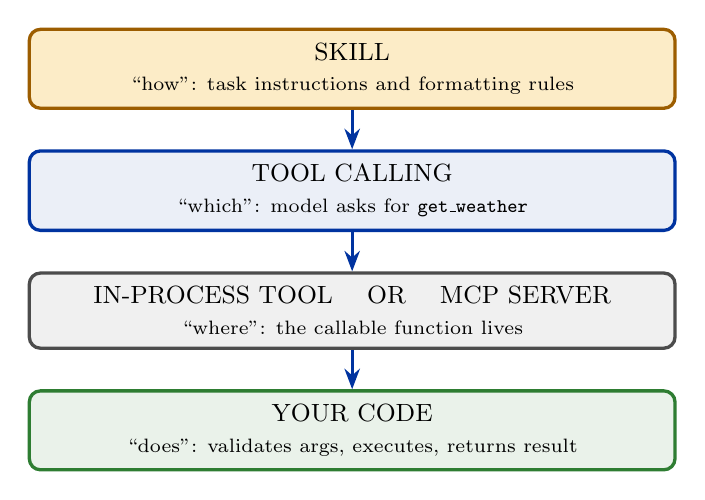
\begin{tikzpicture}[node distance=5mm]
    \node[tserver, minimum width=8.2cm] (skill) {SKILL\\{\scriptsize ``how'': task instructions and formatting rules}};
    \node[tbox, minimum width=8.2cm, below=of skill] (tc) {TOOL CALLING\\{\scriptsize ``which'': model asks for \texttt{get\_weather}}};
    \node[tbox, minimum width=8.2cm, draw=gray!60!black, fill=gray!12, below=of tc] (where) {IN-PROCESS TOOL \quad OR \quad MCP SERVER\\{\scriptsize ``where'': the callable function lives}};
    \node[tcode, minimum width=8.2cm, below=of where] (code) {YOUR CODE\\{\scriptsize ``does'': validates args, executes, returns result}};
    \draw[tflow] (skill) -- (tc);
    \draw[tflow] (tc) -- (where);
    \draw[tflow] (where) -- (code);
  \end{tikzpicture}
  \end{center}
  \footnotesize Each section changes \alert{one layer}. That is the safest way to avoid mixing up tools, MCP, and skills.
\end{frame}

\begin{frame}{One system, four upgrades}
  \small
  \begin{tabular}{@{}p{3.0cm}p{7.2cm}@{}}
    \toprule
    \textbf{Version} & \textbf{What changed from the previous version?} \\
    \midrule
    Direct orchestration & Your code routes the request and calls the function itself. \\
    Tool calling & The model now chooses from a tool menu; your code still executes. \\
    MCP & The same tool moves to a separate server; your app bridges it back to tool calling. \\
    Skills & Task instructions load on demand before the model uses the relevant tool. \\
    \bottomrule
  \end{tabular}
  \vfill
  \begin{block}{Reading strategy}
    \footnotesize Do not memorize four labels. Ask: \alert{who chooses? where does the function live? what instructions were loaded?}
  \end{block}
\end{frame}
% ============================================================ DIRECT
\section{Direct orchestration}

\begin{frame}{Direct orchestration --- the idea}
  \begin{block}{What it is}
    \alert{Your code} owns the control flow. You classify the request, call the right
    function yourself, then (optionally) use the LLM only to phrase the answer. The model
    does \alert{not} choose tools.
  \end{block}
  \footnotesize For our example: \emph{your} code detects ``weather'', extracts ``Yerevan'',
  calls \texttt{get\_weather}, and asks the LLM to phrase the result.
  \begin{columns}[T]
    \column{0.5\textwidth}\textbf{Good when}
      \begin{itemize}\small \item few, known intents \item you want determinism \& low cost \item auditable, testable flow \end{itemize}
    \column{0.5\textwidth}\textbf{Bad when}
      \begin{itemize}\small \item many/open-ended intents \item the routing logic balloons \item you reinvent what tool calling gives free \end{itemize}
  \end{columns}
\end{frame}

\begin{frame}[fragile]{Direct orchestration --- code}
\begin{lstlisting}
def answer(question: str) -> str:
    q = question.lower()
    if "weather" in q or "rain" in q or "umbrella" in q:
        city = extract_city(question)    # regex, form field, or parser
        data = get_weather(city)         # <== KEY: your code picks the tool
        return llm_phrase(question, data)
    if "latest" in q or "today" in q:
        hits = web_search(question)
        return llm_phrase(question, hits)
    return llm_answer(question)           # general knowledge
\end{lstlisting}
\footnotesize \alert{Key line (5):} \emph{your} code decides to call \texttt{get\_weather} --
the model is not involved in the choice. Predictable, but every new capability is another branch.
\end{frame}

\begin{frame}[fragile]{Direct orchestration --- exact trace}
\begin{lstlisting}[style=ascii]
1. user -> app:
   "Will it rain in Yerevan today?"

2. app routes locally:
   q contains "rain" -> choose weather branch

3. app extracts arguments:
   city = "Yerevan"

4. app runs code directly:
   data = get_weather("Yerevan")

5. app asks model only to phrase:
   llm_phrase(question, data)

6. assistant -> user:
   "No rain expected in Yerevan today..."
\end{lstlisting}
\footnotesize The model never chooses a tool here. The decision point is step 2, inside \alert{your code}.
\end{frame}
% ============================================================ TOOL CALLING
\section{Tool calling}

\begin{frame}[fragile]{Tool calling --- the idea}
  \begin{block}{What it is}
    You hand the model a \alert{menu of tools} (JSON schemas). The model replies ``call
    \texttt{get\_weather(city=`Yerevan')}''. \alert{Your code} runs it and feeds the result
    back. The model decides \emph{which} tool and \emph{when}.
  \end{block}
  \begin{center}
  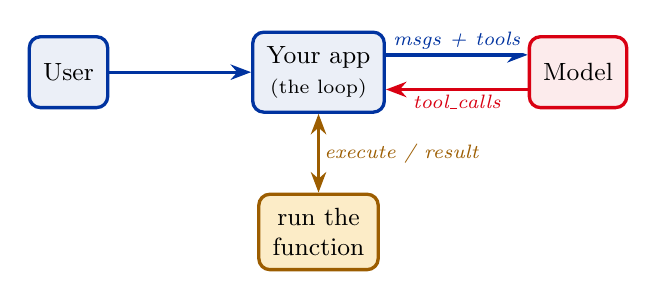
\begin{tikzpicture}[node distance=8mm and 18mm]
    \node[tbox] (user) {User};
    \node[tbox, right=of user] (app) {Your app\\{\scriptsize(the loop)}};
    \node[tmodel, right=of app] (model) {Model};
    \node[tserver, below=10mm of app] (tool) {run the\\function};
    \draw[tflow] (user) -- (app);
    \draw[tflow] ([yshift=2.2mm]app.east) -- node[tlbl,above]{msgs + tools} ([yshift=2.2mm]model.west);
    \draw[tflowR] ([yshift=-2.2mm]model.west) -- node[tlbl,below]{tool\_calls} ([yshift=-2.2mm]app.east);
    \draw[tbi, armorangedark] (app) -- node[tlbl,right]{execute / result} (tool);
  \end{tikzpicture}
  \end{center}
  \footnotesize Every arrow is one HTTP request. A regular answer is just the text path on round 1.
\end{frame}

\begin{frame}[fragile]{Tool calling --- first, the transcript}
  Before SDK code, understand the \alert{message order}:
\begin{lstlisting}[style=ascii]
user:
  Will it rain in Yerevan today?

assistant:
  tool_call id=call_123 name=get_weather args={"city":"Yerevan"}

tool:
  tool_call_id=call_123
  {"condition":"clear sky","temperature_c":20,"wind_kmh":7}

assistant:
  No rain expected in Yerevan today. It is clear and about 20C.
\end{lstlisting}
  \footnotesize The assistant's tool-call message must be in history \alert{before} the tool result, and the result must echo the same \texttt{tool\_call\_id}. (Args shown decoded -- on the wire \texttt{arguments} is a JSON string.)
\end{frame}
\begin{frame}[fragile]{Tool calling --- code (OpenRouter)}
\begin{lstlisting}
client = OpenAI(base_url="https://openrouter.ai/api/v1",
                api_key=os.environ["OPENROUTER_API_KEY"])

tools = [{"type": "function", "function": {
    "name": "get_weather",
    "description": "Current weather for a city.",
    "parameters": {"type": "object",
        "properties": {"city": {"type": "string"}},
        "required": ["city"]}}}]

resp = client.chat.completions.create(model=MODEL, messages=msgs, tools=tools)
msg = resp.choices[0].message
msgs.append(msg.model_dump())              # assistant message with tool_calls
for call in msg.tool_calls or []:
    args = json.loads(call.function.arguments)   # <== KEY: arguments is a STRING
    result = get_weather(**args)                  # your code executes
    msgs.append({"role": "tool", "tool_call_id": call.id,
                 "content": json.dumps(result)})  # id must match
\end{lstlisting}
\footnotesize \alert{Key line (15):} \texttt{arguments} arrives as a JSON \emph{string} -- always
\texttt{json.loads} it. And every \texttt{tool\_call\_id} must echo the call's id.
\end{frame}


\begin{frame}{Tool calling --- gotchas}
  \begin{itemize}
    \item \alert{\texttt{arguments} is a JSON string}, not a dict -- always \texttt{json.loads} it (and guard \texttt{""}).
    \item You must \alert{append the assistant message with \texttt{tool\_calls} before} the tool results.
    \item \alert{Every \texttt{tool\_call\_id} needs exactly one} matching \texttt{tool} message (watch parallel calls).
    \item The model can \alert{hallucinate} tool names/args -- validate before calling \texttt{**args}.
    \item \alert{Cap the rounds} -- tools can loop forever.
    \item \alert{Cost:} the whole tool list is re-sent every round and counts as input tokens.
  \end{itemize}
\end{frame}

% ============================================================ MCP
\section{MCP}

\begin{frame}[fragile]{MCP --- the idea}
  \begin{block}{What it is}
    A \alert{standard protocol} for exposing tools from a \alert{separate server} so any app
    can plug them in (``USB-C for AI''). It does \alert{not} replace tool calling -- the model
    still chooses via tool calling; MCP just standardises where tools live.
  \end{block}
  \begin{center}
  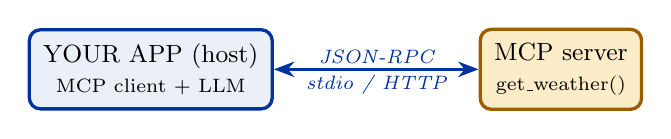
\begin{tikzpicture}[node distance=26mm]
    \node[tbox] (host) {YOUR APP (host)\\{\scriptsize MCP client + LLM}};
    \node[tserver, right=of host] (srv) {MCP server\\{\scriptsize get\_weather()}};
    \draw[tbi, armblue] (host) -- node[tlbl,above]{JSON-RPC} node[tlbl,below]{stdio / HTTP} (srv);
  \end{tikzpicture}
  \end{center}
  \footnotesize Primitives: \alert{tools} (do), \alert{resources} (read), \alert{prompts} (templates).
\end{frame}

\begin{frame}[fragile]{MCP --- server + bridge to OpenRouter}
\begin{lstlisting}
# server.py  -- a standalone tool server (FastMCP)
from mcp.server.fastmcp import FastMCP
mcp = FastMCP("weather")

@mcp.tool()                              # <== KEY: turns a function into a tool
def get_weather(city: str) -> dict:
    """Current weather for a city."""    # docstring+hints -> JSON Schema
    return weather.get_weather(city)
mcp.run()                                  # stdio transport
\end{lstlisting}
\begin{lstlisting}
# client: MCP inputSchema is ALREADY JSON Schema -> near no-op conversion
def mcp_tool_to_openai(t):
    return {"type": "function", "function": {
        "name": t.name, "description": t.description,
        "parameters": t.inputSchema}}  # <== KEY: already JSON Schema
# list_tools() -> convert -> normal OpenRouter loop -> session.call_tool(name, args)
\end{lstlisting}
\footnotesize \alert{Key idea:} the bridge is nearly free -- MCP's \texttt{inputSchema} is already the JSON Schema that tool calling wants.
\end{frame}

\begin{frame}[fragile]{MCP --- exact trace}
\begin{lstlisting}[style=ascii]
SETUP: host connects to the tool server
  1. host starts mcp_server.py over stdio
  2. host creates ClientSession(read, write)
  3. host awaits session.initialize()
  4. host calls session.list_tools()
  5. host converts each inputSchema -> OpenRouter tool schema

USER TURN: normal tool-calling loop
  6. host sends messages + converted tools to the model
  7. model emits get_weather({"city":"Yerevan"})
  8. host routes that call to session.call_tool(...)
  9. MCP server runs weather.get_weather(...)
 10. host appends the tool result and asks the model for final text
\end{lstlisting}
\footnotesize The model only sees ordinary tool calling; MCP is hidden behind the Python host.
\end{frame}

\begin{frame}[fragile]{MCP --- plug in a server you didn't write}
  Because MCP is a standard, you can point the \alert{same bridge} at someone else's server:
\begin{lstlisting}
# our own server:
SERVER = StdioServerParameters(command=sys.executable, args=["mcp_server.py"])

# a third-party server from the web (official "fetch" server, no API key):
SERVER = StdioServerParameters(command="uvx", args=["mcp-server-fetch"])
\end{lstlisting}
  \footnotesize Nothing else changes -- \texttt{list\_tools} $\rightarrow$ convert $\rightarrow$ loop is identical. The model now gets a \texttt{fetch} tool from code we never wrote:
\begin{lstlisting}[style=ascii]
user:  Fetch https://example.com and give the heading.
model: fetch({"url":"https://example.com"})     # tool from a third-party server
tool:  "Example Domain ... for use in documentation examples ..."
model: The heading is "Example Domain".
\end{lstlisting}
  \footnotesize \alert{The payoff of MCP:} reuse existing tool servers instead of writing your own.
\end{frame}

\begin{frame}[fragile]{The key question: tool calling vs MCP}
  They are on \alert{different sides} of your app -- not alternatives.
  \begin{columns}[T]
    \column{0.5\textwidth}
    \begin{block}{Tool calling = app $\leftrightarrow$ model}
      \footnotesize How the \alert{model asks} your app for a function. Built into the LLM
      API. Works with plain Python functions and \alert{zero MCP}.
    \end{block}
    \column{0.5\textwidth}
    \begin{block}{MCP = host/app $\leftrightarrow$ tool server}
      \footnotesize How a host \alert{discovers \& calls} tools in another process,
      vendor-neutrally. The model sees only the converted tool schemas.
    \end{block}
  \end{columns}
  \begin{center}
  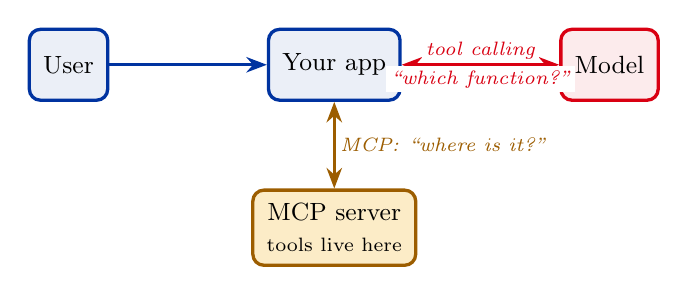
\begin{tikzpicture}[node distance=9mm and 20mm]
    \node[tbox] (user) {User};
    \node[tbox, right=of user] (app) {Your app};
    \node[tmodel, right=of app] (model) {Model};
    \node[tserver, below=11mm of app] (srv) {MCP server\\{\scriptsize tools live here}};
    \draw[tflow] (user) -- (app);
    \draw[tbi, armred] (app) -- node[tlbl,above]{tool calling} node[tlbl,below]{``which function?''} (model);
    \draw[tbi, armorangedark] (app) -- node[tlbl,right]{MCP: ``where is it?''} (srv);
  \end{tikzpicture}
  \end{center}
  \footnotesize MCP tools reach the model \emph{through} tool calling. MCP buys \alert{reuse \& ecosystem}, not a new decision mechanism.
\end{frame}


% ============================================================ SKILLS
\section{Skills (SKILL.md)}

\begin{frame}{Skills --- the idea}
  \begin{block}{What it is}
    A folder with a \texttt{SKILL.md} (instructions) + optional scripts/files, loaded
    \alert{on demand}. It packages \emph{know-how}, not capabilities. (Anthropic feature;
    \alert{OpenRouter has no native skills} -- you port the \emph{pattern}.)
  \end{block}
  \begin{alertblock}{The key distinction}
    \footnotesize A \alert{tool} lets the assistant \emph{do} something. A \alert{skill} tells the assistant \emph{how} to do it well.
  \end{alertblock}
  \begin{block}{Progressive disclosure (the whole point)}
    \footnotesize
    \begin{tabular}{@{}lll@{}}
      \textbf{Level 1} & name + description & always (\textasciitilde100 tokens each) \\
      \textbf{Level 2} & full SKILL.md body & only when triggered \\
      \textbf{Level 3} & bundled files/scripts & only when referenced \\
    \end{tabular}
  \end{block}
  \footnotesize 100 skills cost \textasciitilde100 tokens each up front; heavy content loads only when needed.
\end{frame}

\begin{frame}[fragile]{Skills --- what changes in the answer}
\begin{lstlisting}[style=ascii]
without a skill:
  model -> get_weather("Yerevan") -> generic weather answer

with weather-lookup skill:
  model -> load_skill("weather-lookup")
        -> read formatting rules
        -> get_weather("Yerevan")
        -> yes/no first, then humidity and wind
\end{lstlisting}
  \vfill
  \footnotesize The capability is still \texttt{get\_weather}. The skill changes the \alert{procedure and output standard}.
\end{frame}
\begin{frame}[fragile]{Strict skills --- exact trace}
\begin{lstlisting}[style=ascii]
START OF TURN: only one tool is visible
  tools=[load_skill]
  system prompt lists skill names + descriptions only

1. user -> app:
   "Should I bring an umbrella in Yerevan?"

2. model -> app:
   load_skill({"name":"weather-lookup"})

3. app -> model as tool result:
   full SKILL.md body
   [Tools now available: get_weather]

4. next model round sees:
   tools=[load_skill, read_skill_file, get_weather]

5. model -> app:
   get_weather({"city":"Yerevan"})

6. model writes final answer using the loaded instructions
\end{lstlisting}
\footnotesize Strict mode forces the \alert{path}: instruction first, capability second. It still cannot guarantee perfect adherence.
\end{frame}
\begin{frame}[fragile]{SKILL.md --- format + porting to OpenRouter}
\begin{lstlisting}[style=ascii]
---
name: weather-lookup
description: Fetches weather and formats it. Use when the user asks about
  weather, temperature, rain, "should I bring an umbrella", ...
allowed-tools: [get_weather]          # which tools this skill needs
---
# Weather Lookup
1. Call get_weather with the city. 2. Lead with one plain sentence. ...
\end{lstlisting}
  \textbf{Porting the pattern (no native support):}
  \begin{itemize}\footnotesize
    \item put only each skill's \alert{name+description} in the system prompt;
    \item give the model a \alert{\texttt{load\_skill(name)}} tool that returns the full body on demand;
    \item \alert{Flat} = domain tools always available (model may skip \texttt{load\_skill}).
          \alert{Strict} = tools \emph{locked} until a skill unlocks them (forces the path).
  \end{itemize}
\end{frame}

\begin{frame}{Skills --- gotchas}
  \begin{itemize}
    \item \alert{Vague descriptions never trigger} -- the description is the entire match surface. Be specific, third-person, with the words a user would say.
    \item \alert{Enforcement $\neq$ adherence:} you can force \texttt{load\_skill} to run, but a weak model may still ignore the instructions it loaded.
    \item \alert{Specific instructions can still fail} -- e.g. ``do not add a year to search queries'' may be ignored by a weak model.
    \item \alert{Skills are instructions, not magic} -- effectiveness is capped by the model.
    \item Keep \texttt{SKILL.md} small; push detail into bundled files (loaded on demand).
    \item \alert{Security:} bundled scripts run with your permissions -- audit them.
  \end{itemize}
\end{frame}

% ============================================================ CHOOSING
\section{Choosing}

\begin{frame}[fragile]{They are layers, not competitors}
  \begin{center}
  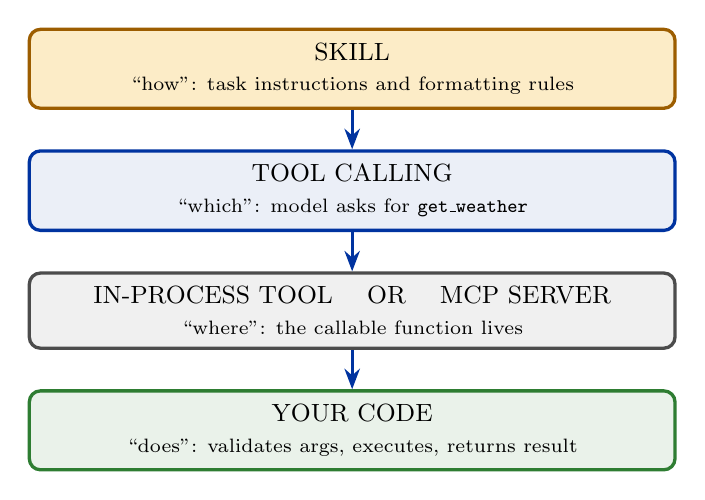
\begin{tikzpicture}[node distance=5mm]
    \node[tserver, minimum width=8.2cm] (skill) {SKILL\\{\scriptsize ``how'': task instructions and formatting rules}};
    \node[tbox, minimum width=8.2cm, below=of skill] (tc) {TOOL CALLING\\{\scriptsize ``which'': model asks for \texttt{get\_weather}}};
    \node[tbox, minimum width=8.2cm, draw=gray!60!black, fill=gray!12, below=of tc] (wh) {IN-PROCESS TOOL \quad OR \quad MCP SERVER\\{\scriptsize ``where'': the callable function lives}};
    \node[tcode, minimum width=8.2cm, below=of wh] (code) {YOUR CODE\\{\scriptsize ``does'': validates args, executes, returns result}};
    \draw[tflow] (skill) -- (tc);
    \draw[tflow] (tc) -- (wh);
    \draw[tflow] (wh) -- (code);
  \end{tikzpicture}
  \end{center}
  \footnotesize \alert{Same four layers as the start.} A skill sets \emph{how}; tool calling picks \emph{which};
  the function lives in-process or over \emph{MCP}; and \emph{your code} does the work. Each approach changes
  \alert{one layer} -- direct orchestration just skips the model's choice.
\end{frame}

\begin{frame}{The same question, four ways}
  \small ``Will it rain in Yerevan today?''
  \begin{itemize}
    \item \textbf{Direct orchestration:} \emph{your code} detects ``weather'', calls \texttt{get\_weather(``Yerevan'')}, LLM phrases.
    \item \textbf{Tool calling:} the \emph{model} emits \texttt{get\_weather(city=``Yerevan'')}; your code runs it; the model answers.
    \item \textbf{MCP:} same model-facing tool call, but \texttt{get\_weather} lives in a \alert{separate server}; the host routes the call there.
    \item \textbf{Skills:} the model loads the \texttt{weather-lookup} skill (formatting rules), \emph{then} calls \texttt{get\_weather}, and answers in the skill's style.
  \end{itemize}
  \vfill
  \footnotesize Same five-step shape; what changes is \alert{who decides} and \alert{where the tool lives}.
\end{frame}

\begin{frame}{Side-by-side comparison}
  \scriptsize
  \begin{tabular}{@{}p{2.1cm}p{1.7cm}p{1.7cm}p{1.7cm}p{3.2cm}@{}}
    \toprule
    & \textbf{Direct orch.} & \textbf{Tool calling} & \textbf{MCP} & \textbf{Skills} \\
    \midrule
    Who decides      & code        & model        & model        & model (picks the skill) \\
    Tools live       & in-process  & in-process   & sep. server  & n/a (instructions) \\
    Loaded up front  & all logic   & all schemas  & all schemas  & \alert{only descriptions} \\
    Setup cost       & low         & low          & \alert{high} & medium \\
    Reuse across apps& no          & no           & \alert{yes}  & yes (portable md) \\
    Best for         & few/known flows & open-ended choice & shared tools & many instruction sets \\
    \bottomrule
  \end{tabular}
  \vfill
  \footnotesize All four can co-exist in one assistant.
\end{frame}

\begin{frame}{Decision guide --- when to use which}
  \begin{itemize}
    \item \alert{Few, well-known flows; want determinism} $\rightarrow$ \textbf{direct orchestration}.
    \item \alert{Open-ended; let the model pick among tools} $\rightarrow$ \textbf{tool calling} (start here for most assistants).
    \item \alert{Reuse tools across apps / use the ecosystem} $\rightarrow$ \textbf{MCP} (otherwise plain functions are simpler).
    \item \alert{Many task-specific instruction sets; context is filling up} $\rightarrow$ \textbf{skills}.
  \end{itemize}
  \vfill
  \begin{block}{Pragmatic path}
    \footnotesize Build with plain \alert{tool calling} first. Add \alert{MCP} only when a tool
    needs to be shared. Add \alert{skills} only when the system prompt gets bloated. Use
    \alert{direct orchestration} for the narrow, must-be-correct paths.
  \end{block}
\end{frame}

\begin{frame}{Bridge to text-to-SQL}
  The same architecture shows up in the internship SQL assistant:
  \vfill
  \begin{tabular}{@{}p{3.1cm}p{3.5cm}p{3.5cm}@{}}
    \toprule
    & \textbf{Weather toy} & \textbf{Text-to-SQL} \\
    \midrule
    Tool & \texttt{get\_weather(city)} & \texttt{run\_sql(query)} \\
    Direct orchestration & code detects weather & code runs classify $\rightarrow$ generate SQL $\rightarrow$ execute/repair \\
    Tool calling / MCP & model asks for weather & model asks to run SQL and can recover from results/errors \\
    Skill & weather answer style & SQL procedure, safety rules, answer style \\
    \bottomrule
  \end{tabular}
  \vfill
  \begin{block}{Important implication}
    \footnotesize For SQL, the quality lift usually comes from the \alert{execution-feedback loop}
    (run $\rightarrow$ inspect result/error $\rightarrow$ repair), not from MCP by itself.
  \end{block}
\end{frame}

\begin{frame}{Cross-cutting engineering footnotes}
  \begin{itemize}
    \item \alert{Logging silently broken:} a later \texttt{basicConfig} is a no-op if the root logger is already configured (use \texttt{force=True}).
    \item \alert{Trusting docs over the installed version:} an SDK class in the docs may not exist in the release -- introspect what's installed.
    \item \alert{Forgetting to cache} a geocode/weather call $\rightarrow$ hammering a free tier.
    \item \alert{Letting one bad turn crash the REPL} -- wrap each turn; keep the session alive.
  \end{itemize}
\end{frame}

\begin{frame}{Summary}
  \begin{itemize}
    \item One idea: \alert{model decides, your code does}.
    \item \textbf{Direct orchestration} -- code routes; simple, rigid.
    \item \textbf{Tool calling} -- model routes; the foundation everything builds on.
    \item \textbf{MCP} -- tool calling + a standard plug for \alert{reusable} tool servers (different side of the app, not a replacement).
    \item \textbf{Skills} -- on-demand \alert{instructions} via progressive disclosure.
  \end{itemize}
  \vfill
  \begin{block}{Rule of thumb}
    \footnotesize Start with tool calling. Add MCP only when a tool must be shared across apps.
    Add skills only when the system prompt gets bloated. Use direct orchestration for the
    narrow, must-be-correct paths.
  \end{block}
  \vfill
  \centering \alert{Questions?}
\end{frame}

\end{document}
